% \lstset{style=mystyle}
\section{ALU}
In the section we will focus on the ALU in the RISC-V architecture by explaining in detail how it works. The ALU is the arithmetic logic unit and in the context of this project, it will only do multiplication and division operations. 
\begin{figure}[H]
                \centering
                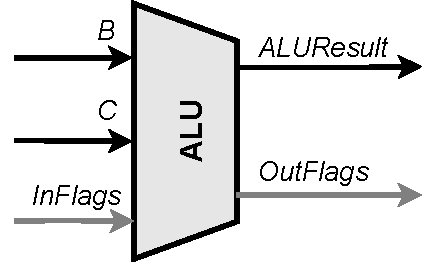
\includegraphics[width=.6\columnwidth]{pics/diagrams/riscv/modules/alu}
                \caption{ALU overview}\
\end{figure}
\subsection{Overview}
For an operation to be executed, the ALU receives a bit value from the control unit to indicate which operation to execute. As for the inputs, the ALU receives from the register file with the flags. For both operations, the ALU will first change the inputs to their absolute values.
\begin{code}{Assigning Absolute value operation}
wire [lv:0] AbsA;
AbsoluteValue #(l) abs_a(
	.A(A), .R(AbsA)
);
wire [lv:0] AbsB;
AbsoluteValue #(l) abs_b(
	.A(B), .R(AbsB)
);
\end{code}

According to the operation intended, the ALU will import the flags necessary. In case of multiplication, the ALU will update the value of multiplication overflow flag. 

\begin{code}{Assigning multiplication operation}
1: begin
    // Multiplication
    UnsignedR = MultiplicationR;
    FlagsOut[MultiplicationOverflowIdx[lv:0]] =
    MultiplicationOverflow | SignOverflow;
    FlagsOut[DivisionHasRemainderIdx[lv:0]] =                  FlagsIn[DivisionHasRemainderIdx[lv:0]];
    FlagsOut[DivisionByZeroIdx[lv:0]] =  FlagsIn[DivisionByZeroIdx[lv:0]];
    FlagsOut[DivisionOverflowIdx[lv:0]] = FlagsIn[DivisionOverflowIdx[lv:0]];
end
\end{code}

In our case when the operation wire has 1 then that indicates that a multiplication operation should be executed.
In the case of a division, there are two flags to be updated: divisionHasRemainder, which will indicate a remainder, and divisionDivByZero, which will indicate the edge case of division by zero. 

\begin{code}{Assigning division operation}
0: begin
// Division
UnsignedR = DivisionR;
FlagsOut[DivisionHasRemaindeFlagOut[lv:0]] = DivisionHasRemainder;
FlagsOut[DivisionByZeroFlagOut[lv:0]] = DivisionDivByZero;
FlagsOut[DivisionOverflowFlagOut[lv:0]] = SignOverflow;
FlagsOut[MultiplicationOverflowFlagOut[lv:0]] = FlagsIn[MultiplicationOverflowFlagOut[lv:0]];
end
\end{code}

In case of no flags are raised the noFlagsIdx. %not sure how it works
After doing the operation between two unsigned integers. The ALU operates to give a sign to the result.

\begin{code}{Sign operation}
reg [lv:0] UnsignedR;
wire SignOverflow;
GiveSign #(l) give_sign(
	.Sign(A[lv] ^ B[lv]),
	.A(UnsignedR),
	.R(R),
	.Overflow(SignOverflow)
);
\end{code}

The overall structure can be seen in Figure \ref{fig:alu_structure}:
\begin{figure}[H]
    \centering
    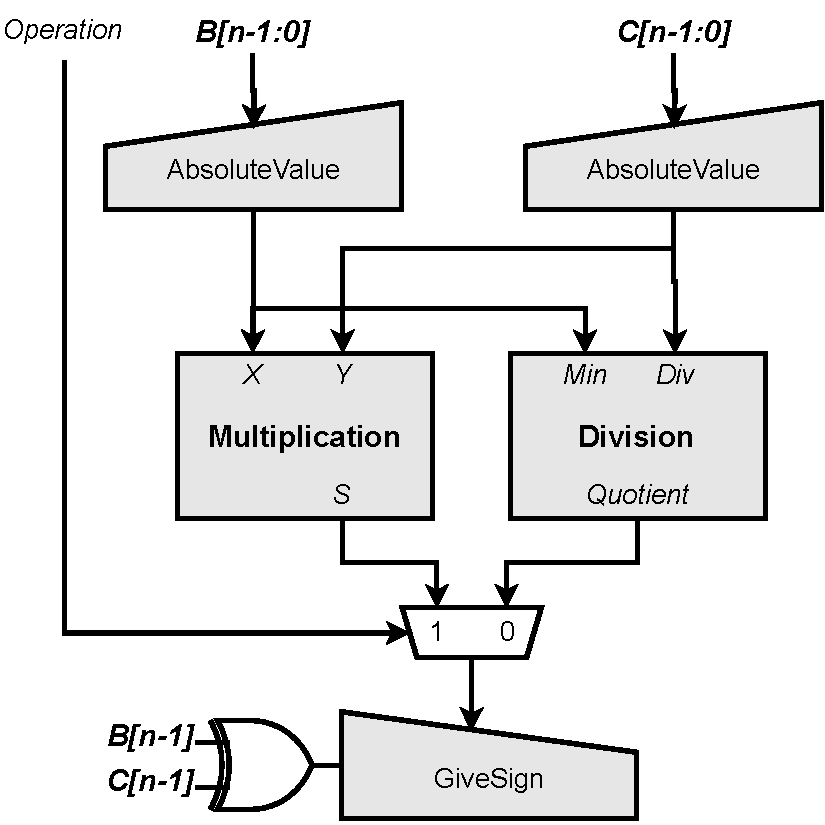
\includegraphics[width=.8\columnwidth]{pics/diagrams/riscv/modules/alu_structure}
    \caption{ALU structure}
    \label{fig:alu_structure}
\end{figure}

\subsection{Addition}
\begin{code}{1 bit adder}
module Adder (
	input X,
	input Y,
	input Cin,
	output S,
	output Cout
);

assign S = X ^ Y ^ Cin;
assign Cout = (X & Y) | ((X ^ Y) & Cin);

endmodule //Adder
\end{code}
We start by implementing one bit adder. Then we use it to implement a full adder for 16 bits.
\begin{code}[14]{Full adder }
module FullAdder #(parameter l = 16) (
	input [lv:0] X,
	input [lv:0] Y,
	input Cin,
	output [lv:0] S,
	output [lv:0] Cout
);

parameter lv = l-1;

wire [lv:0] Sum;
wire [l:0] Cout_temp;
assign Cout_temp[0] = Cin;

// Remaining bits
generate genvar i;
	for (i = 0; i <= lv; i = i + 1) begin
		Adder adder(X[i], Y[i], Cout_temp[i], Sum[i], Cout_temp[i+1]);
	end
endgenerate

assign S = Sum;
assign Cout[lv:0] = Cout_temp[l:1];

endmodule //FullAdder
\end{code}
We reimplement this full adder to make a full adder with overflow and carry flag. Overflow in case the addition of two positive number became negative because the range of bits representing the integers was exceeded. Carry in case the range of bits to represent the number was exceeded.
\begin{code}[49]{Full adder with flags}
module FullAdderFlags #(parameter l = 16) (
	input [lv:0] X,
	input [lv:0] Y,
	output [lv:0] S,
	output Overflow,
	output Carry
);

parameter lv = l-1;

wire [lv:0] Cout;

FullAdder #(l) full_adder (
	.X(X), .Y(Y), .Cin(1'b0),
	.S(S), .Cout(Cout)
);

assign Overflow = Cout[lv-1] ^ Cout[lv];
assign Carry = Cout[lv];

endmodule // FullAdderFlags
\end{code}
\subsection{Multiplication}
The multiplication is a composition of the addition operation and shift. That was the approach used, make the multiplication operation through the addition block we created.
In order for the multiplication to work we just copy the multiplier whenever we find a 1, then shift or skip and shift when we find a zero. We only add carries in the next operation for optimization purposes. So we do an addition operation then we add the result to the next addition operation and we add the carry too. That is the general concept. However, to optimize this operation, each time we shift we add the bits on the right to the final result and we keep going until the operation is finished. The result will be represented in 32 bit but we only compute the first 16 bits the second half is discarded and if it has some value in it then it is an overflow. These operations will be further explained one by one in the next sub-subsections.
Of course there are certain edge cases like carry and overflow which have specific flags to be raised when they happen.
\begin{figure}[H]
                \centering
                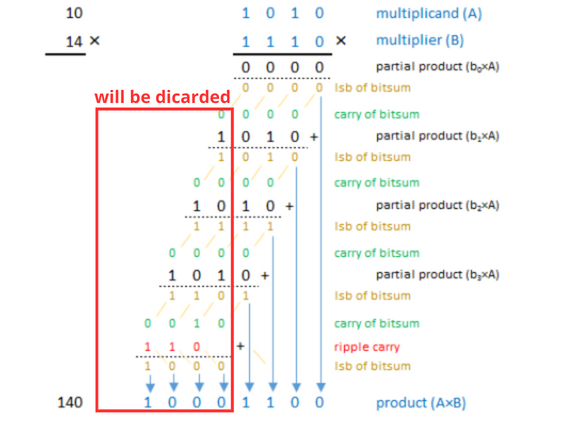
\includegraphics[width=.5\textwidth]{pics/multiplicationOp.png}
                \caption{Multiplication}\
\end{figure}
\subsubsection{Contolled adder circuit}
The controlled adder is the same as the 1 bit adder. As a matter of fact it uses the 1 bit adder we created only with one twist. we add another input to this controlled adder which is selection. This input will specify if we preceed with the addition or we ignore it and shift. In our case if the inpur is 1, we will preceed with the addition and if it is 0 we skip.\\
The figure below illustrate the diagram of controlled adder, as x, y, cin and selection are the inputs and cout and S are the outputs.
\begin{figure}[H]
                \centering
                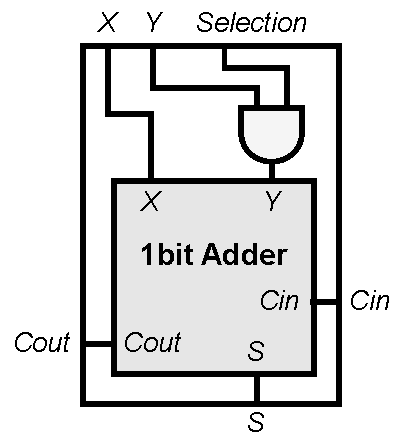
\includegraphics[width=.2\textwidth]{pics/diagrams/multiplication/controlled_adder.pdf}
                \caption{Controlled adder diagram}\
\end{figure}
\subsubsection{Contolled full adder circuit}
The controlled full adder circuit is the collection of the controller adder, which will allow us to do the same operation for 16 bits. So we just use the controlled adder multiple time. As for the carry we do not care about it as it will be passed to the next full adder. In other words cout for each controlled adder will not be connected to the next one rather to the one below it as shown in 3.3.3. This way we are multiplying one bit from the multiplier with all bits of the multiplicand.
\begin{figure}[H]
                \centering
                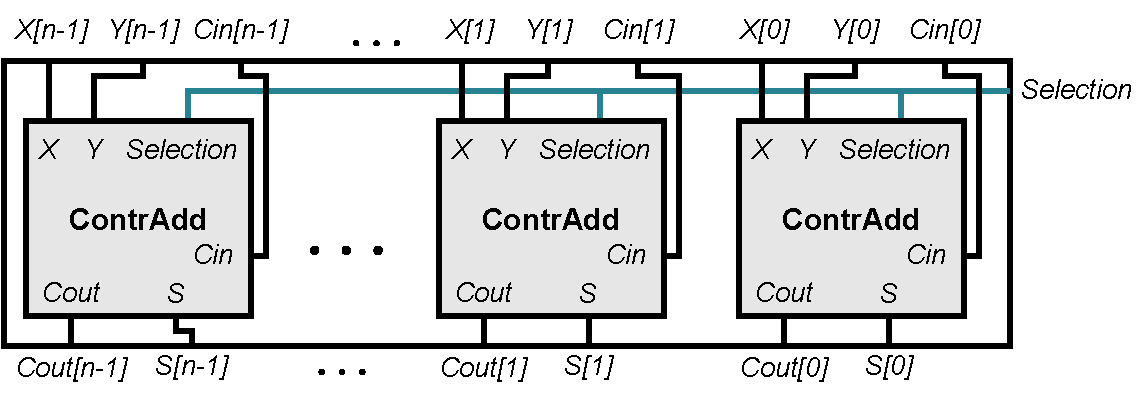
\includegraphics[width=.5\textwidth]{pics/diagrams/multiplication/controlled_full_adder.pdf}
                \caption{Controlled full adder diagram}\
\end{figure}
\subsubsection{Multiplication circuit}
Now we need to do the same operation of the controlled full adder 16 times.
This way we are multiplying each bit of the multiplier with all bits of the multiplicand. The result will be 32 bits. That is why we only compute the first 16 bits as we consider any bit out of that range overflow.\\
As shown in the simplified diagram below, if we are dealing with a 3 bit operation. The result will be 6 bits but we only compute the first 3 and we take the rest of the bits and the carry, we compare it with 0 to decide if there is a carry or an overflow.  
\begin{figure}[H]
                \centering
                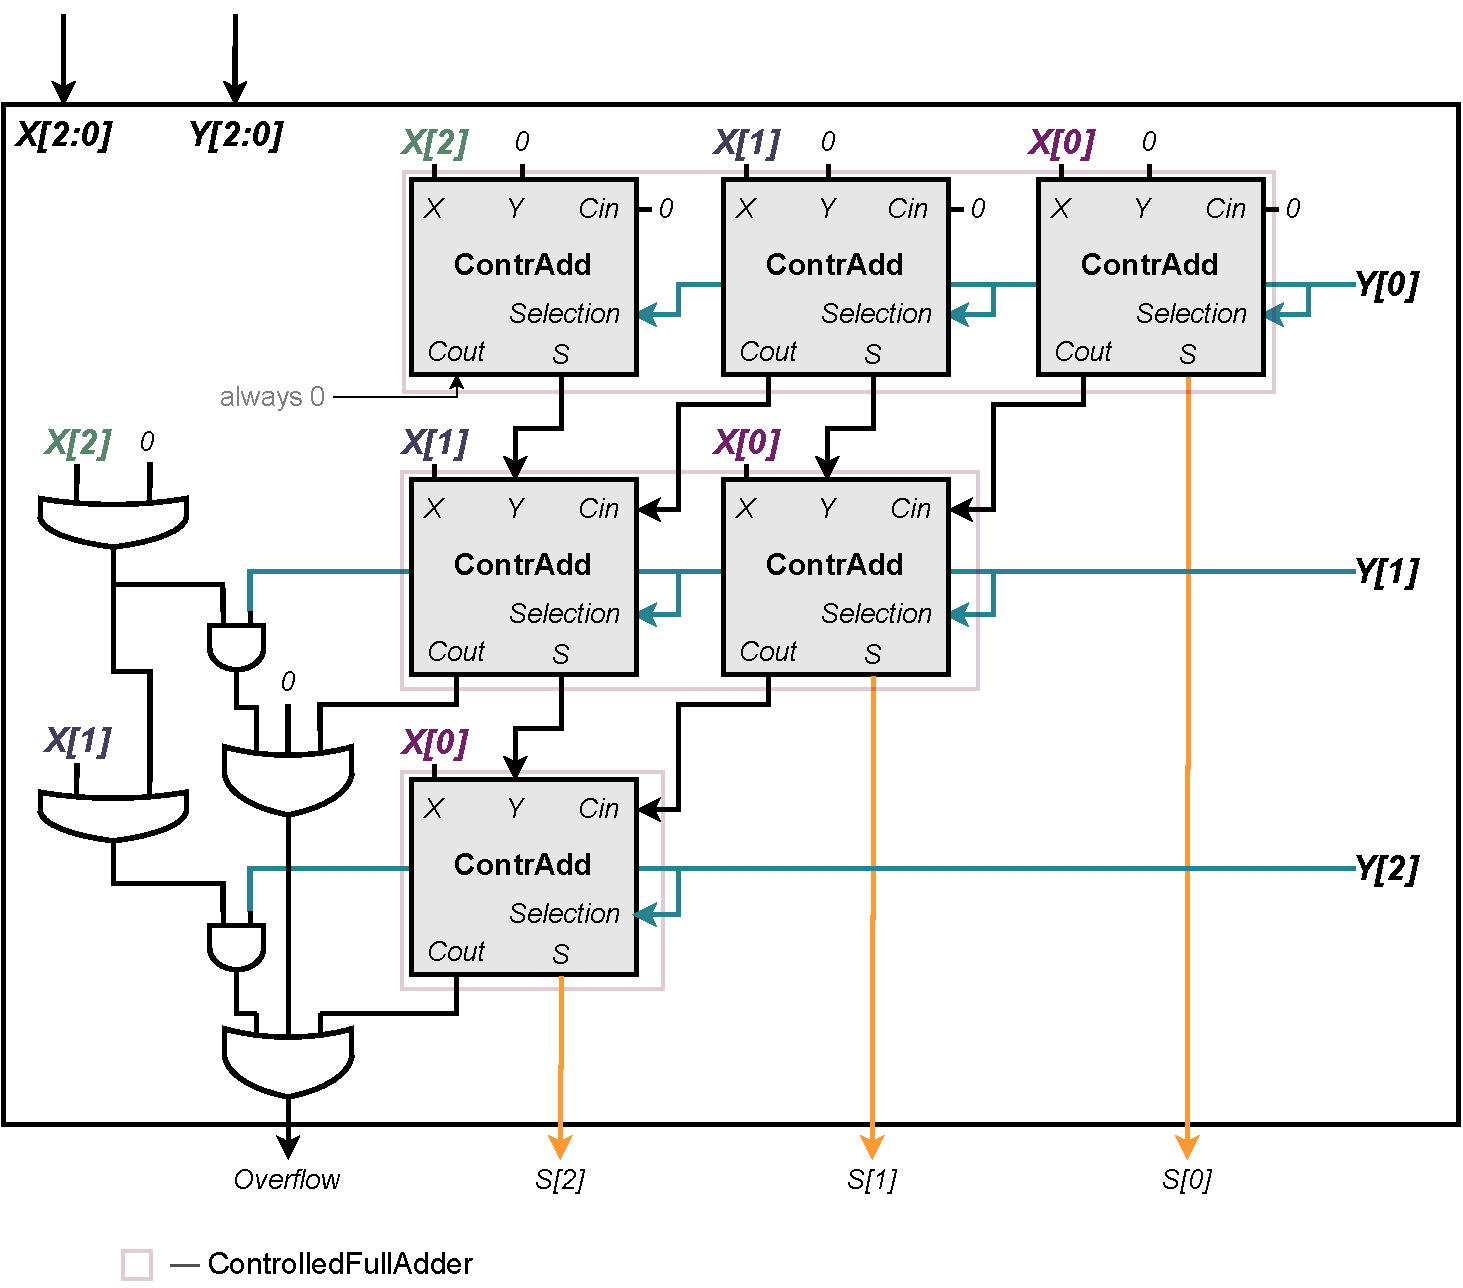
\includegraphics[width=.5\textwidth]{pics/diagrams/multiplication/multiplication.pdf}
                \caption{Multiplication diagram}
\end{figure}


\subsection{Division}
The division works similarly to the multiplication but with some changes. The division is a composition of the subtraction and shift operation.
That was the approach used, make the division operation through the subtraction block we created.
In order for the division to work we just copy the divider whenever we find a 0 in the borrow, then shift or skip and shift when we find a 1. So we do a subtraction operation then we shift and add the result to the next subtraction operation. That is the general concept. We created flags for division by zero and remainder. So for each case, a flag will be raised.
The division will be discussed in more detail in the next sub-subsections.
\begin{figure}[H]
                \centering
                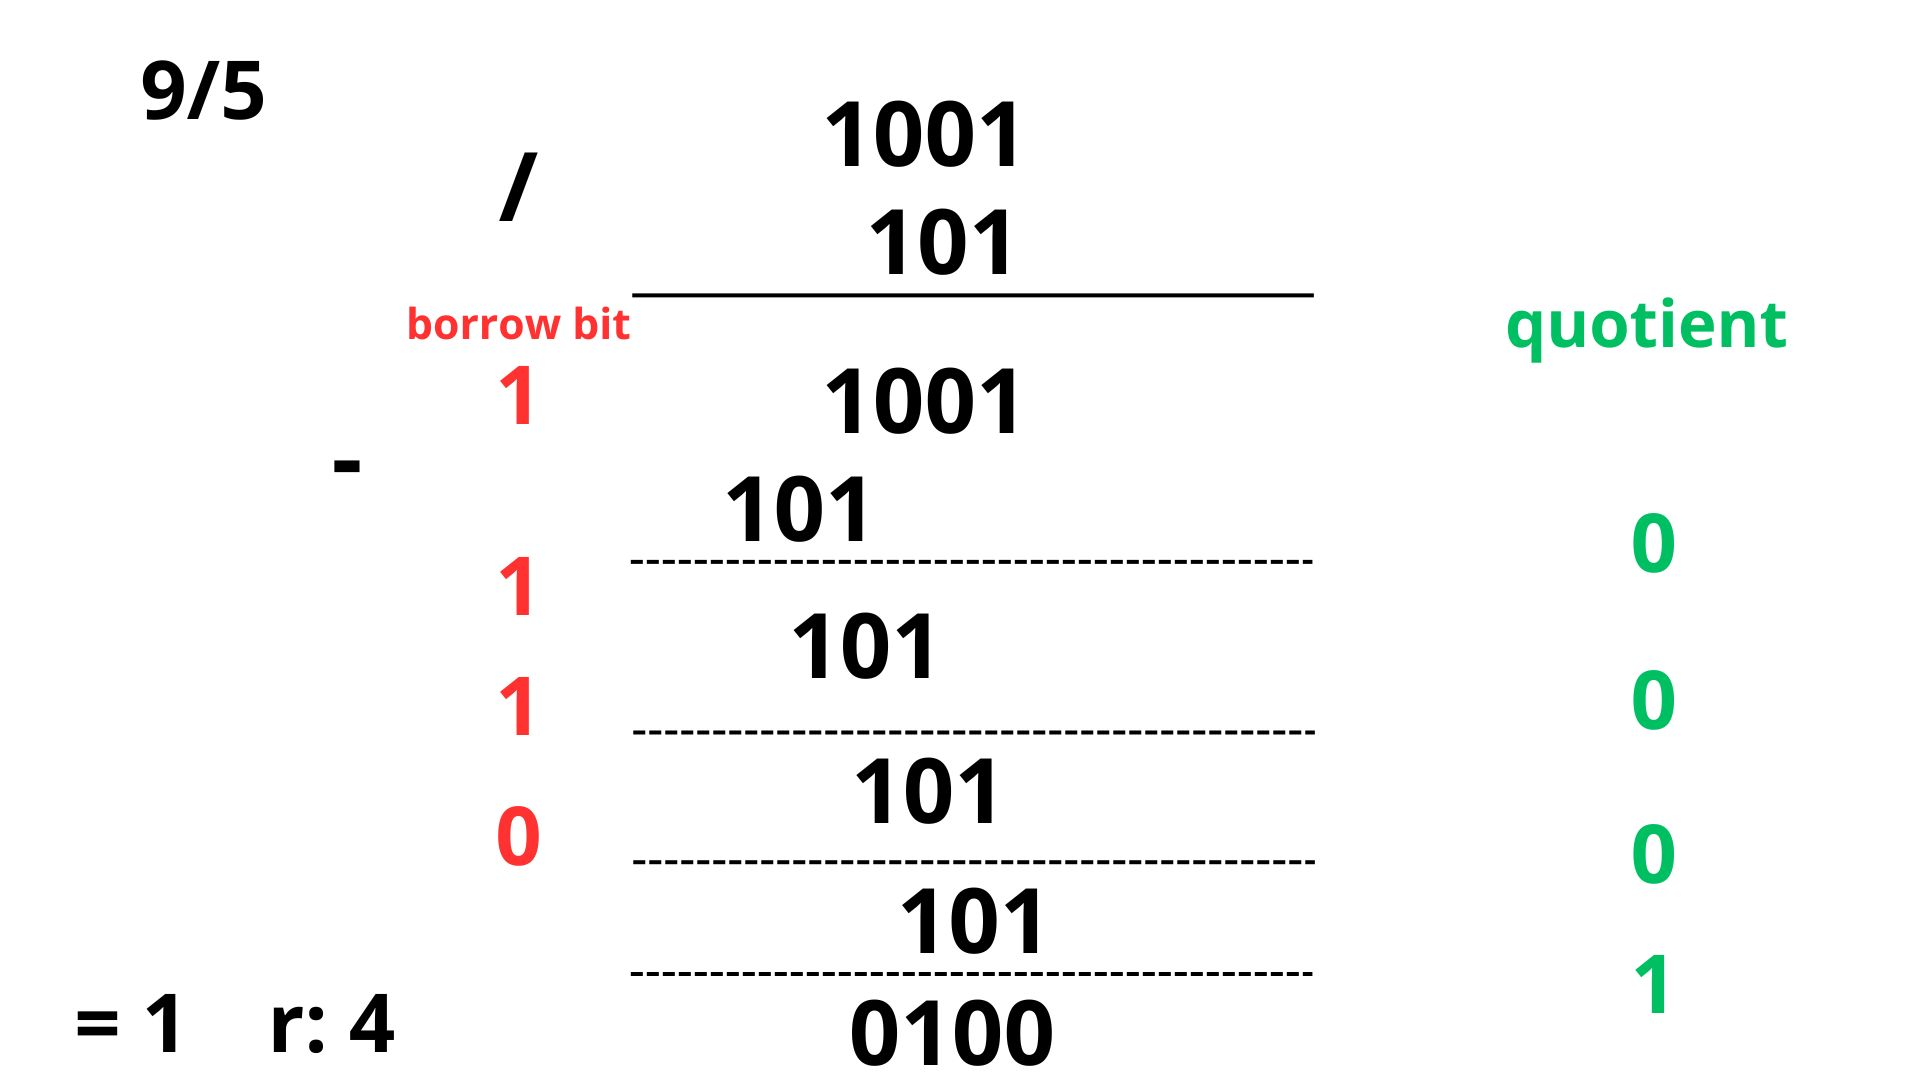
\includegraphics[width=.5\textwidth]{pics/devOp.jpg}
                \caption{Division}\
\end{figure}
\subsubsection{Subtractor}
This block is to subtract one bit from another.
To implement the subtraction we  use the following formulas:
\begin{align*}
D &= A \oplus B \oplus \text{Bin} \\
Bout &= (\neg A \land B) \lor ((\neg (A \oplus B)) \land \text{Bin})
\end{align*}
\subsubsection{Controlled subtractor}
The controlled subtractor, just like the controlled addition, is the same as a subtractor but with a small addition, which is the Selection input as shown in the diagram. Unlike the controlled addition, when the selection input is 0, the difference will be output as the difference. However when the selection is 1, the minuend will be out as the difference.
\begin{figure}[H]
                \centering
                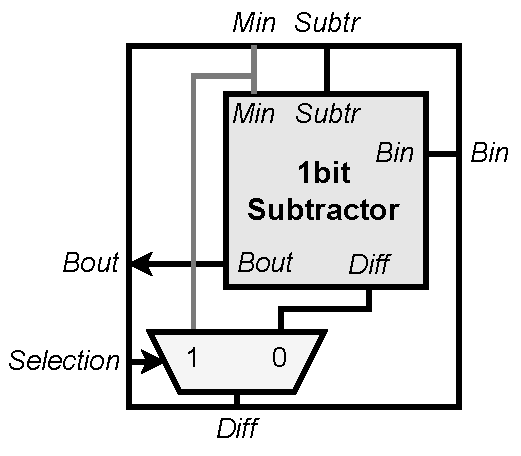
\includegraphics[width=.3\textwidth]{pics/diagrams/division/controlled_subtractor.pdf}
                \caption{Controlled subtractor diagram}\
\end{figure}
\subsubsection{Controlled full subtractor}
The controlled full substractor in the  collection of controlled subtractors. They are linked through the borrow out and borrow in as each borrow out becomes the borrow in of the next block. As shown in the figure, the output of the borrow out (Bout) will be forwarded to selection to determine if the output of the difference will be the difference or the minuend as explained in the previous sub-subsection. The Bout of the most significant bit is negated to form the quotient. If there is no borrow then the subtraction is possible and then the quotient bit in that block is 1 if not the the bit is 0. 
\begin{figure}[H]
                \centering
                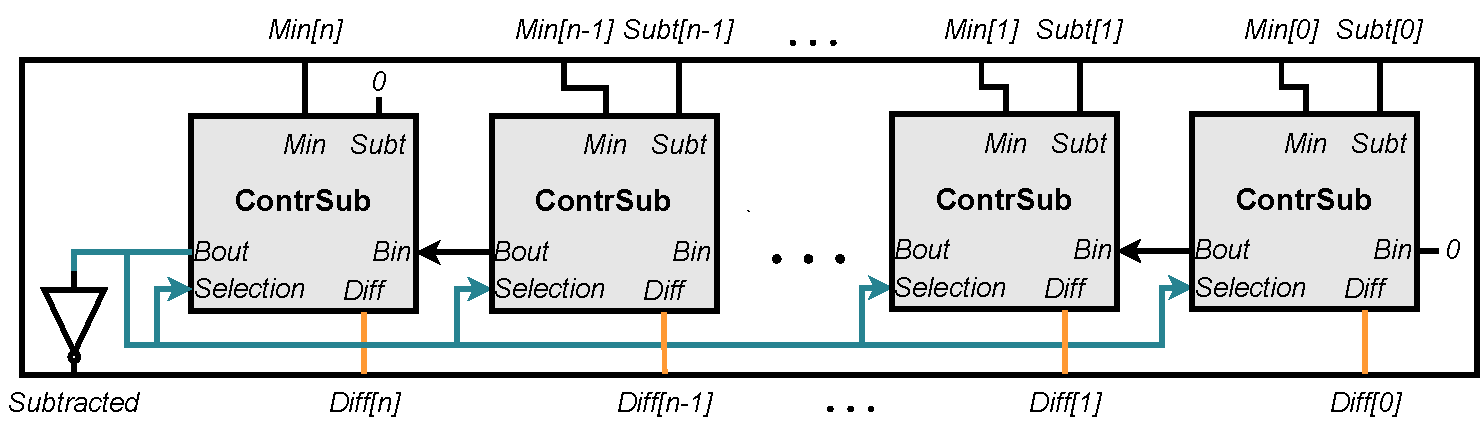
\includegraphics[width=.5\textwidth]{pics/diagrams/division/controlled_full_subtractor.pdf}
                \label{fig:controlled_full_subtractor}
                \caption{Controlled subtractor diagram}\
\end{figure}
\subsubsection{Division}
\begin{figure*}[!t]
    \centering
    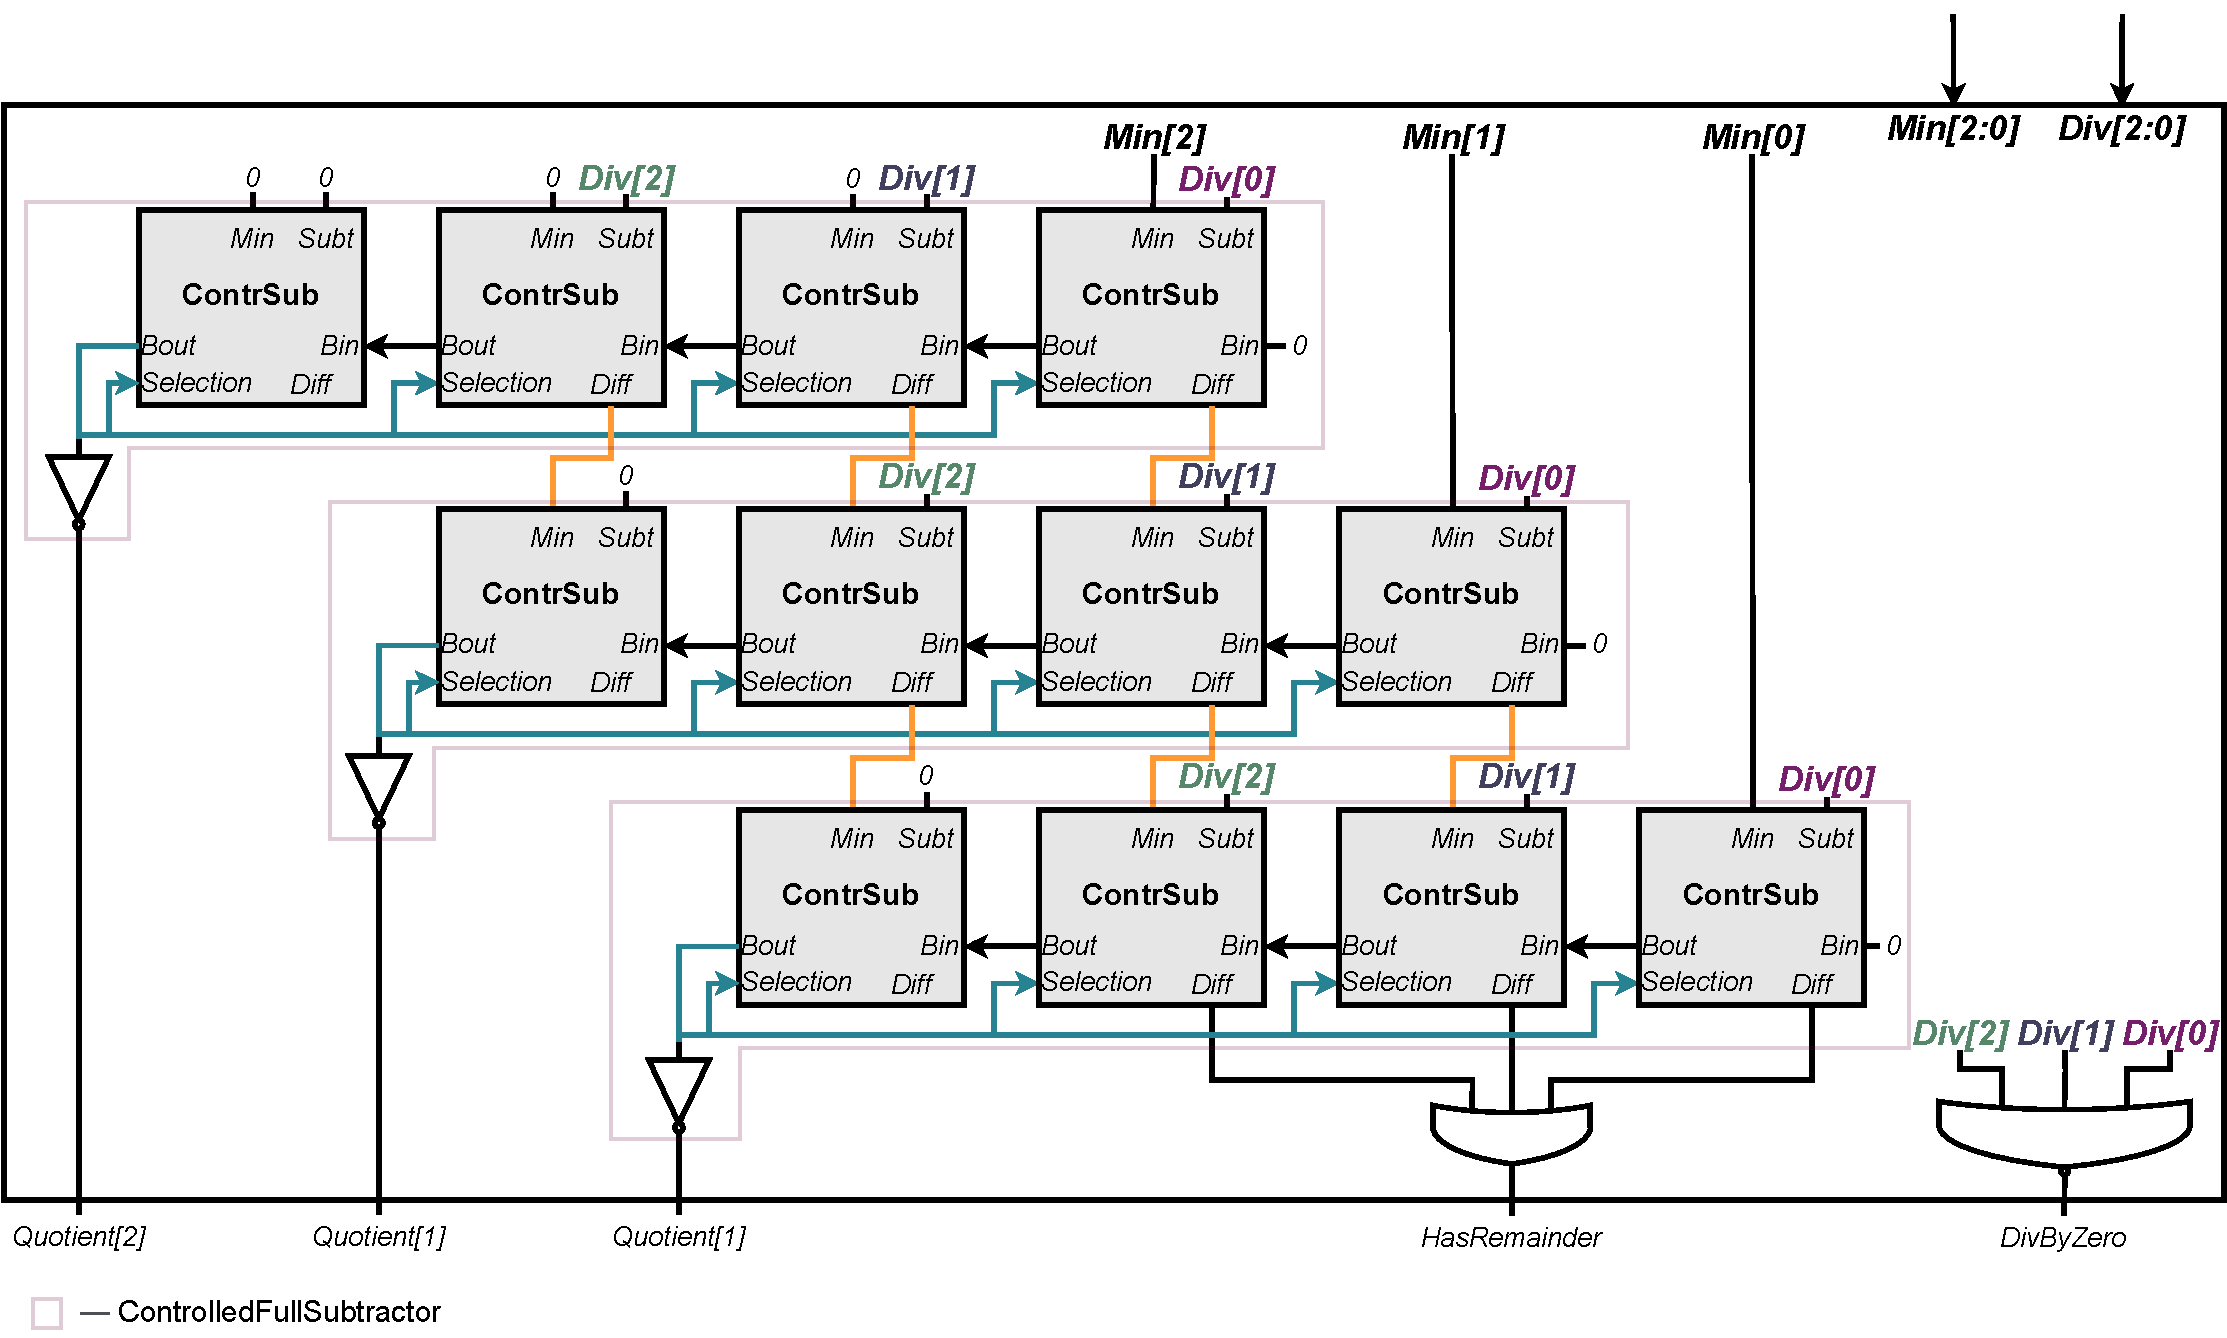
\includegraphics[width=.8\textwidth]{pics/diagrams/division/division}
    \caption{Division diagram}
    \label{fig:division}
\end{figure*}

Finally, to form the division operation, the combination of multiple layers of controlled full subtractor will result in the division operation. In the Figure \ref{fig:division} below, we can see a simplified division operation for two 3-bit integers. It is clear how the shift happens from layer to layer and within each layer, a bit from the minuend is included as input. the last block in the first layer is not an input block but rather a block so the most significant bit finds from where to borrow. The difference is forwarded from layer to layer bit by bit until it reached the end of the division where it will be forwarded to hasRemainder. If it is not 0 then the flag will be raised. Also if the divider is 0 it will also raise DivByzero. That is why we have NOR to check if we have a 000 or not.

